\qrchapter{https://forgottenpillar.com/rsc/en-fp-chapter10}{Is God a person? - by John N. Loughborough}


\qrchapter{https://forgottenpillar.com/rsc/es-fp-chapter10}{¿Es Dios una persona? - por John N. Loughborough}


One of the earliest articles on the \emcap{personality of God} is Loughborough’s article “\textit{Is God a person?}” where he discusses the \emcap{personality of God} and His presence. It is important to remember the definition of ‘personality’ according to the Merriam-Webster dictionary: “\textit{the quality or state of being a person}”\footnote{\href{https://www.merriam-webster.com/dictionary/personality}{Merriam-Webster Dictionary - ‘\textit{personality}’}}. We will look carefully at how Loughborough sees the quality or state of God being a person.


Uno de los primeros artículos sobre la \emcap{personalidad de Dios} es el artículo de Loughborough “¿\textit{Es Dios una persona?}” donde habla de la \emcap{personalidad de Dios} y su presencia. Es importante recordar la definición de ‘personalidad’ según el diccionario Merriam-Webster: “\textit{la cualidad o estado de ser una persona}”\footnote{\href{https://www.merriam-webster.com/dictionary/personality}{Diccionario Merriam-Webster - ‘\textit{personalidad}’}}. Vamos a ver detenidamente cómo ve Loughborough la cualidad o estado de Dios siendo una persona.


\begin{figure}[hp]
    \centering
    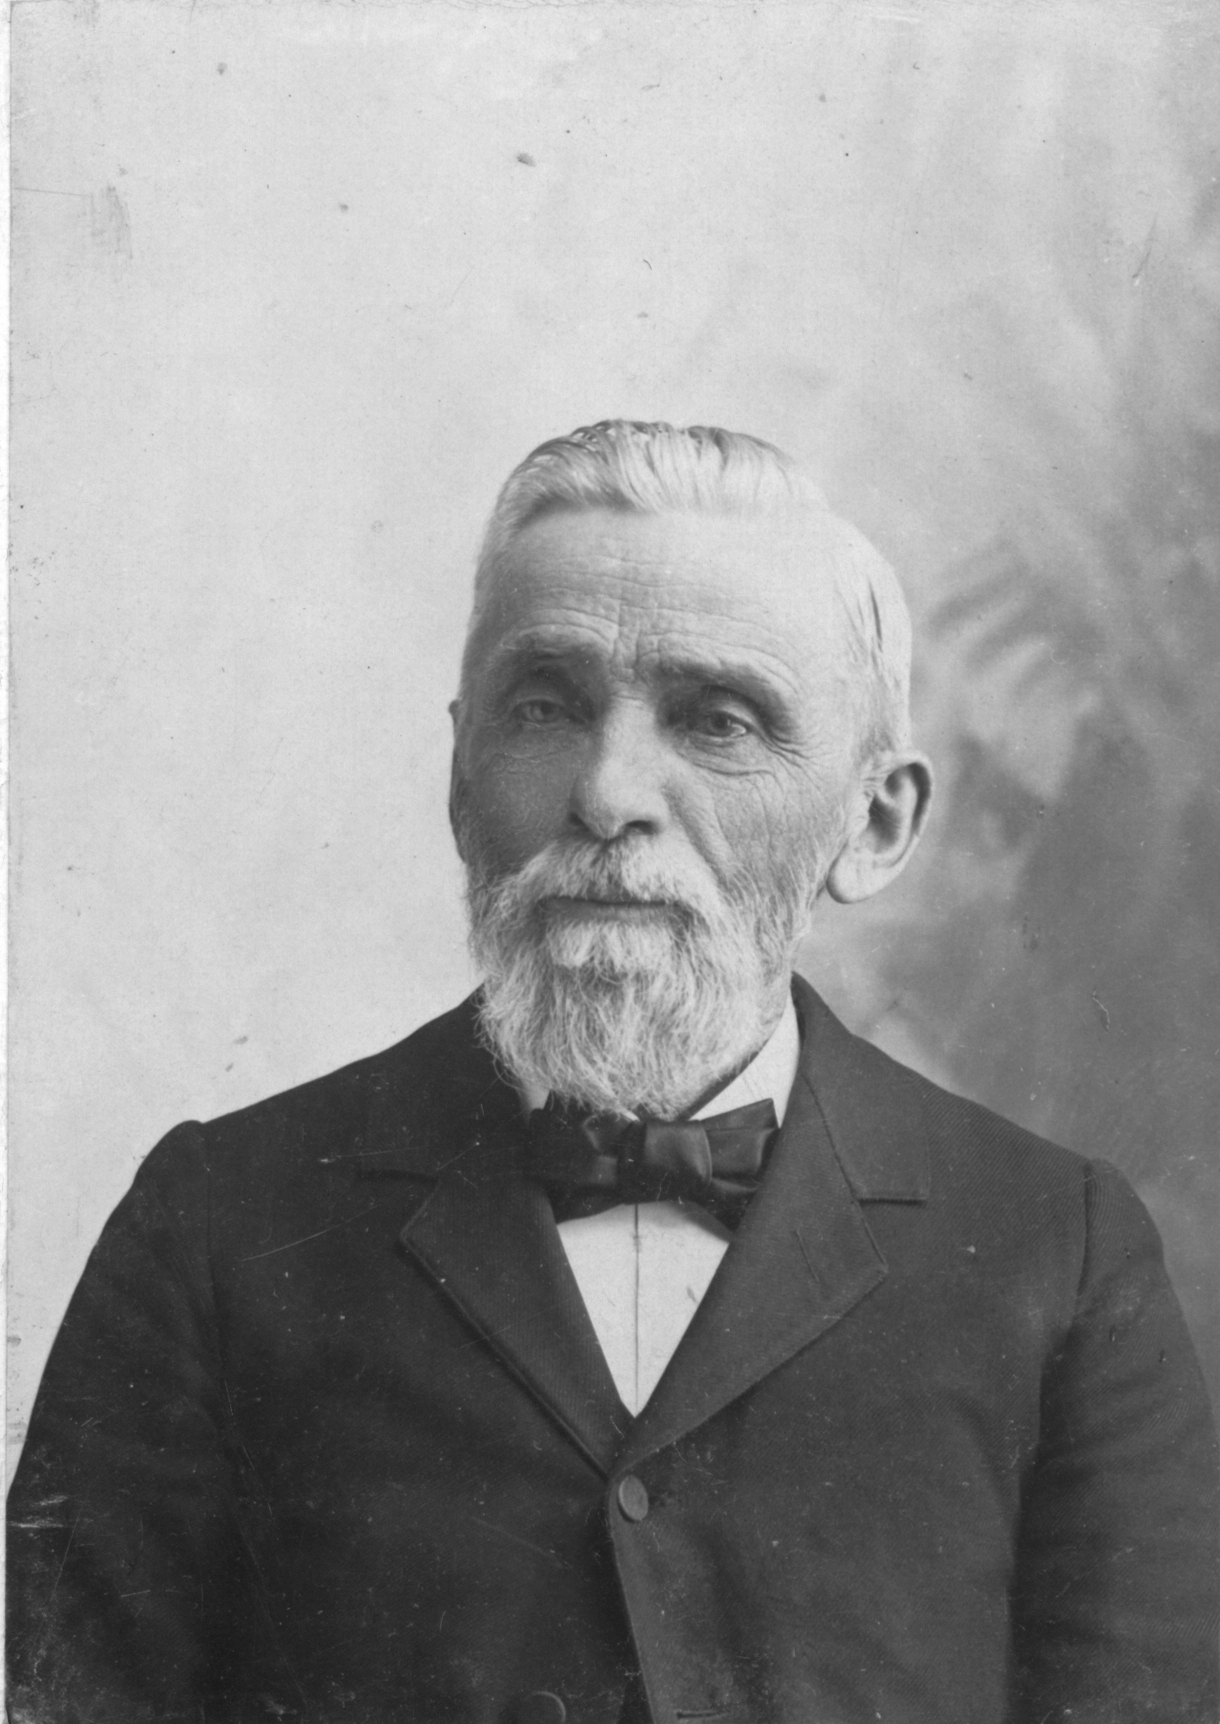
\includegraphics[width=1\linewidth]{images/john-n-loughborough.jpg}
    \caption*{John Norton Loughborough (1832-1924)}
    \label{fig:john-n-loughborough}
\end{figure}


\begin{figure}[hp]
    \centering
    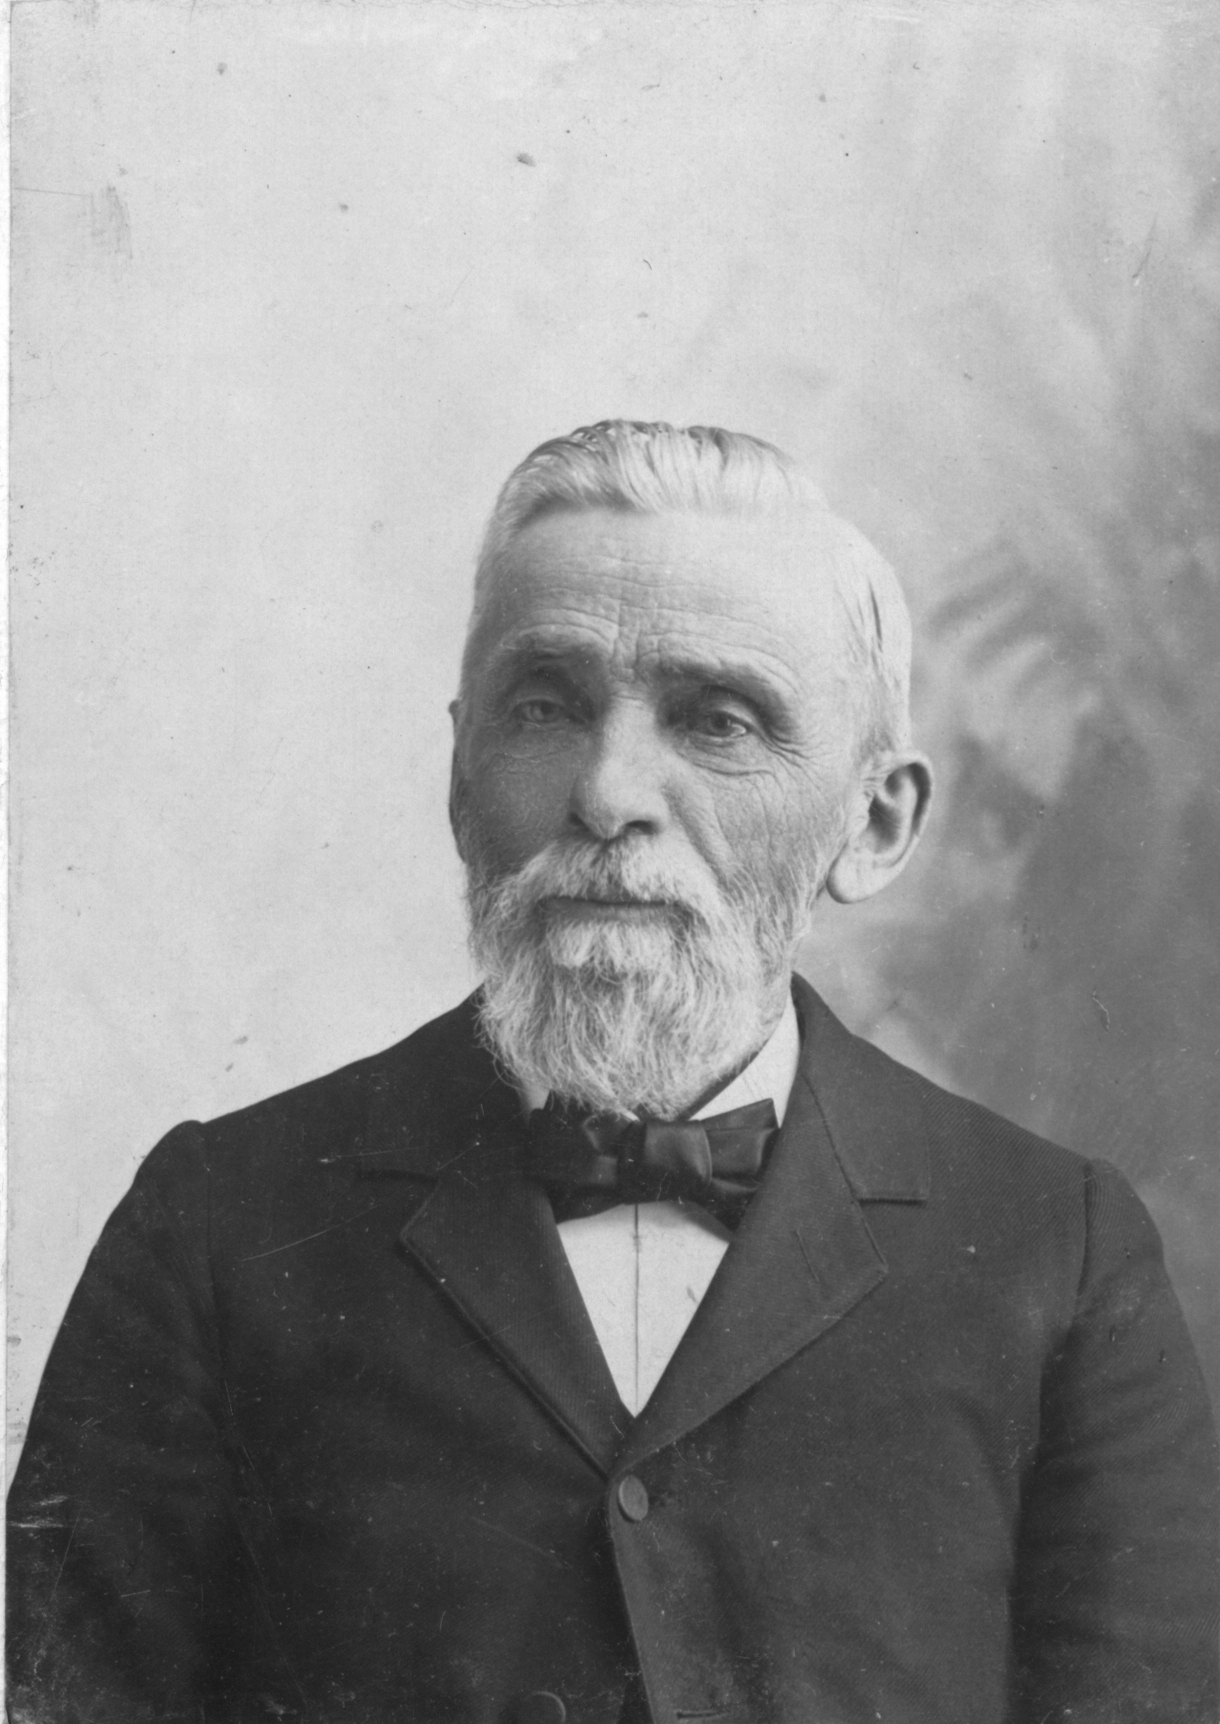
\includegraphics[width=1\linewidth]{images/john-n-loughborough.jpg}
    \caption*{John Norton Loughborough (1832-1924)}
    \label{fig:john-n-loughborough}
\end{figure}


\others{Whatever may be the truth in this matter, it certainly cannot be wrong for us to examine what the Word says respecting it. \textbf{Many there are that would refrain from the investigation of unpopular truths because the cry of heresy is raised against them}. We shall not consider ourselves subjects of the appellation, \textbf{neither are we prying into the secrets of the Almighty, as we pursue the investigation of this matter}. The Bible certainly contains testimony upon this point, and we again repeat, ‘\textbf{Things which are revealed belong to us}.’ We inquire then, What saith the Scripture?}


\others{Sea cual sea la verdad en este asunto, ciertamente no puede ser malo que examinemos lo que la Palabra dice al respecto. \textbf{Hay muchos que se abstendrían de investigar las verdades impopulares porque se levanta el grito de herejía contra ellas}. No nos consideraremos sujetos de ese apelativo, \textbf{ni estaremos entrometiéndonos en los secretos del Todopoderoso, al proseguir la investigación de este asunto}. La Biblia contiene ciertamente un testimonio sobre este punto, y repetimos de nuevo: ‘\textbf{Las cosas reveladas nos pertenecen}’. Preguntamos entonces, ¿Qué dice la Escritura?}


\othersnogap{\textbf{The very testimony we have been examining in regard to man’s being formed of the dust in \underline{the image of God}, proves conclusively that \underline{God has a form}, although the sentiment is contrary to what we have been taught, while children, from the catechism}:}


\othersnogap{\textbf{El mismo testimonio que hemos estado examinando con respecto a que el hombre fue formado del polvo a \underline{la imagen de Dios}, demuestra de manera concluyente que \underline{Dios tiene una forma}, aunque el sentimiento es contrario a lo que se nos ha enseñado, cuando éramos niños, en el catecismo}:}


\othersnogap{Question. ‘What is God?’}


\othersnogap{Pregunta. ‘¿Qué es Dios?’}


\othersnogap{Answer. ‘An infinite and eternal spirit; one that always was and always will be.’}


\othersnogap{Respuesta. ‘Un espíritu infinito y eterno; que siempre fue y siempre será’.}


\othersnogap{Q. ‘Where is God?’}


\othersnogap{P. ‘¿Dónde está Dios?’}


\othersnogap{A. ‘Everywhere.’}


\othersnogap{R. ‘En todas partes.’}


\othersnogap{\textbf{But we inquire, \underline{Is not God in one place more than another}?} Oh no, say you: \textbf{the Bible says \underline{he is a spirit}, and if so he must be \underline{everywhere alike}}. Well, if when man dies his spirit goes to God, it must go everywhere. \textbf{But the Bible certainly represents God as located in heaven. ‘For he hath looked down from the height of his sanctuary: from heaven did the Lord behold the earth.’ Psalm 102:19}. \textbf{Then certainly heaven cannot be everywhere, for God is represented as looking down from it. ‘\underline{Elijah went up} by a whirlwind \underline{into heaven}.’ 2 Kings 2:11}. \textbf{But, says one, does not the Bible represent God \underline{as everywhere present}?} Psalm 139:8, 9, 10. ‘If I ascend up into heaven, \textbf{thou art there}: if I make my bed in hell, \textbf{behold, thou art there}; if I take the wings of the morning, and dwell in the uttermost parts of the sea,\textbf{ even there shall thy hand lead me}, and thy right hand shall hold me.’}


\othersnogap{\textbf{Pero nosotros preguntamos, \underline{¿No está Dios en un lugar más que en otro}?} Oh no, decís vosotros: \textbf{la Biblia dice \underline{que es un espíritu}, y si es así debe estar \underline{en todas partes por igual}}. Bueno, si cuando el hombre muere su espíritu va a Dios, debe ir a todas partes. \textbf{Pero la Biblia ciertamente representa a Dios como ubicado en el cielo. ‘Porque desde la altura de su santuario miró hacia abajo; desde el cielo contempló el Señor la tierra’. Salmo 102:19}. \textbf{Entonces, ciertamente el cielo no puede estar en todas partes, porque Dios es representado como mirando hacia abajo desde él. ‘\underline{Elías subió} por un torbellino \underline{al cielo}’. 2 Reyes 2:11}. \textbf{Pero, dice uno, ¿no representa la Biblia a Dios como \underline{presente en todas partes}?} Salmo 139:8, 9, 10. ‘Si subo al cielo, \textbf{allí estás tú}; si hago mi cama en el infierno, \textbf{allí estás tú}; si tomo las alas del alba y habito en los confines del mar, \textbf{allí me llevará tu mano}, y me sostendrá tu diestra.’}


\othersnogap{We reply, \textbf{the subject is introduced in verse 7, as follows}: ‘\textbf{\underline{Whither shall I go from thy Spirit}?} \textbf{or whither shall I flee from \underline{thy presence}?}’ \textbf{The Spirit is \underline{God’s representative}}. \textbf{His power is manifested wherever he listeth, through the agency of his Spirit}. Christ, when giving the commission to the disciples, says, ‘Go ye into all the world, and preach the gospel to every creature, and lo! \textbf{I am with you alway, even unto the end of the world}.’ Now, no one would contend that Christ had been on the earth personally ever since the disciples commenced to fulfill this commission. \textbf{But his Spirit has been on the earth; the Comforter that he promised to send.} \textbf{So in the same manner God manifests himself \underline{by his Spirit} which is also the power through which he works}. ‘But if \textbf{the Spirit of him} that raised up Jesus from the dead dwell in you, \textbf{he that raised up Christ} from the dead shall also quicken your mortal bodies \textbf{\underline{by his Spirit} that dwelleth in you}.’ Romans 8:11. \textbf{\underline{Here is a plain distinction made between the Spirit, and God that raises the dead by that Spirit}}. \textbf{If the living God is a Spirit in the strictest sense of the term, and at the same time is in possession of a Spirit, then we have at once the novel idea of the Spirit of a Spirit, something it will take at least a Spiritualist to explain}.}[The Adventist Review and Sabbath Herald, September 18, 1855][https://documents.adventistarchives.org/Periodicals/RH/RH18550918-V07-06.pdf]


\othersnogap{Respondemos, \textbf{el tema se introduce en el versículo 7, de la siguiente manera}: ‘\textbf{\underline{¿Adónde me iré de tu Espíritu}?} \textbf{o ¿a dónde huiré de \underline{tu presencia}?}’ \textbf{El Espíritu es \underline{el representante de Dios}}. \textbf{Su poder se manifiesta dondequiera que él quiera, por medio de la agencia de su Espíritu}. Cristo, al dar la comisión a los discípulos, dice: ‘Id por todo el mundo y predicad el evangelio a toda criatura, y he aquí, \textbf{yo estoy con vosotros todos los días, hasta el fin del mundo}’. Ahora bien, nadie sostendría que Cristo ha estado en la tierra personalmente desde que los discípulos comenzaron a cumplir esta comisión. \textbf{Pero su Espíritu ha estado en la tierra; el Consolador que prometió enviar.} \textbf{De la misma manera Dios se manifiesta \underline{por su Espíritu} que es también el poder por el cual obra}. ‘Pero si \textbf{el Espíritu de aquel} que resucitó a Jesús de entre los muertos habita en vosotros, \textbf{aquel que resucitó a Cristo} de entre los muertos vivificará también vuestros cuerpos mortales \textbf{\underline{por su Espíritu} que habita en vosotros}’. Romanos 8:11. \textbf{\underline{Aquí se hace una clara distinción entre el Espíritu y Dios que resucita a los muertos por ese Espíritu}}. \textbf{Si el Dios viviente es un Espíritu en el sentido más estricto del término, y al mismo tiempo está en posesión de un Espíritu, entonces tenemos de inmediato la novedosa idea del Espíritu de un Espíritu, algo que tomará por lo menos un espiritista para explicar}.}[The Adventist Review and Sabbath Herald, September 18, 1855][https://documents.adventistarchives.org/Periodicals/RH/RH18550918-V07-06.pdf]


Allow us to make a short comment. We hope you recognize the specific topic being discussed here. The subject is the first point of the \emcap{Fundamental Principles} and the assertion is that God does have a form, for man is made in the image of God. Such understanding of God’s personality precludes the idea that God is everywhere present. Brother Loughborough gave the biblical reasons for God's omnipresence, together with the sentiment that “\textit{God is in one place more than another}”. God is everywhere present by His representative, the Holy Spirit, just as it is written in the first point of the \emcap{Fundamental Principles}. Further in this discussion, we will read that God is a spiritual being and possesses a tangible, material body, in contrast to the idea that He is purely a spirit.


Permítanos hacer un breve comentario. Esperamos que usted reconozca el tema específico que se discute aquí. El tema es el primer punto de los \emcap{Principios Fundamentales} y la afirmación es que Dios sí tiene una forma, pues el hombre está hecho a imagen de Dios. Tal comprensión de la personalidad de Dios excluye la idea de que Dios está presente en todas partes. El hermano Loughborough dio las razones bíblicas de la omnipresencia de Dios, junto con el sentimiento de que “\textit{Dios está en un lugar más que en otro}”. Dios está presente en todas partes por medio de su representante, el Espíritu Santo, tal como está escrito en el primer punto de los \emcap{Principios Fundamentales}. Más adelante en esta discusión, leeremos que Dios es un ser espiritual y posee un cuerpo tangible y material, en contraste con la idea de que Él es puramente un espíritu.


\others{There is at least one impassable difficulty in the way of \textbf{those who believe \underline{God is immaterial}, and heaven is not a literal, \underline{located place}: they are obliged to admit that \underline{Jesus is there bodily, a literal person}}; the same Jesus that was crucified, dead, and buried, was raised from the dead, \textbf{ascended up to heaven}, and is now \textbf{at the right hand of God}. \textbf{Jesus was possessed of flesh and bones after his resurrection}. Luke 24:39. ‘\textbf{Behold my hands and my feet, that it is I, myself; handle me, and see; \underline{for a spirit hath not flesh and bones as ye see me have}}.’ \textbf{If Jesus is there in heaven with a literal body of flesh and bones, may not heaven after all be a literal place, a habitation for a literal God, a literal Saviour, literal angels, and resurrected immortal saints?} \textbf{\underline{Oh no, says one, ‘God is a Spirit.’}} So Christ said to the woman of Samaria at the well. \textbf{It does not necessarily follow because God is a Spirit, \underline{that he has no body}}. In John 3:6, Christ says to Nicodemus, ‘\textbf{That which is born of the Spirit is spirit}.’ \textbf{If that which is born of the Spirit is spirit, then on the same principle, that which has a spiritual nature is spirit. God is \underline{a spirit being}, his nature is spirit, he is not of a mortal nature; }\textbf{\underline{but this does not exclude the idea of his having a body}}. David says, [Psalm 114:4,] ‘Who maketh \textbf{his angels spirits};’ yet \textbf{\underline{angels have bodies}}. Angels appeared to both Abraham and Lot, and ate with them. \textbf{We see the idea that angels are spirits, does not prove that they are not literal beings}.}


\others{Hay al menos una dificultad infranqueable en el camino de \textbf{aquellos que creen que \underline{Dios es inmaterial}, y que el cielo no es un lugar literal y \underline{localizado}: están obligados a admitir que \underline{Jesús está allí corporalmente, una persona literal}}; el mismo Jesús que fue crucificado, muerto y enterrado, fue resucitado de entre los muertos, \textbf{ascendió al cielo}, y está ahora \textbf{a la derecha de Dios}. \textbf{Jesús fue poseído de carne y huesos después de su resurrección}. Lucas 24:39. ‘\textbf{Mirad mis manos y mis pies, que soy yo mismo; palpad y ved; \underline{porque un espíritu no tiene carne y huesos como veis que tengo yo}}’. \textbf{Si Jesús está allí en el cielo con un cuerpo literal de carne y huesos, ¿no será el cielo, después de todo, un lugar literal, una morada para un Dios literal, un Salvador literal, ángeles literales y santos inmortales resucitados?} \textbf{\underline{Oh no, dice uno, ‘Dios es un Espíritu.’}} Así dijo Cristo a la mujer de Samaria en el pozo. \textbf{No se deduce necesariamente que porque Dios sea un Espíritu, \underline{no tenga cuerpo}}. En Juan 3:6, Cristo le dice a Nicodemo: ‘\textbf{Lo que ha nacido del Espíritu es espíritu}’. \textbf{Si lo que ha nacido del Espíritu es espíritu, entonces, por el mismo principio, lo que tiene una naturaleza espiritual es espíritu. Dios es \underline{un ser espiritual}, su naturaleza es espiritual, no es de naturaleza mortal; }\textbf{\underline{pero esto no excluye la idea de que tenga un cuerpo}}. David dice, [Salmo 114:4,] ‘Quien hace \textbf{a sus ángeles espíritus};’ sin embargo, \textbf{\underline{los ángeles tienen cuerpos}}. Los ángeles se aparecieron tanto a Abraham como a Lot, y comieron con ellos. \textbf{Vemos que la idea de que los ángeles son espíritus, no prueba que no sean seres literales}.}


\othersnogap{It is inferred because the Bible says that God is a Spirit, that he is not a person. An inference should not be made the basis for an argument. Great Scripture truths are plainly stated, and it will not do for us to found a doctrine on inferences, \textbf{contrary to positive statements in the word of God}. If the Scripture states in positive \textbf{terms that God is a person, it will not answer for us to draw an inference from the text which says ‘God is a Spirit,’ \underline{that he has no body}}.}


\othersnogap{Se infiere porque la Biblia dice que Dios es un Espíritu, que no es una persona. Una inferencia no debe ser la base de un argumento. Las grandes verdades de la Escritura están claramente declaradas, y no nos servirá fundar una doctrina en inferencias, \textbf{contrarias a las declaraciones positivas en la palabra de Dios}. Si la Escritura afirma en términos \textbf{positivos} que Dios es una persona, no nos servirá sacar una inferencia del texto que dice ‘Dios es un Espíritu’, \underline{que no tiene cuerpo}.}


\othersnogap{We will now present a few texts \textbf{which prove that God is a person}. Exodus 33:18, 23. ‘And he (Moses) said, I beseech thee shew me thy glory.’ Verse 20. ‘And he said, \textbf{Thou canst not see \underline{my face}, for there shall no man see me and live}.’ Verses 21-23. ‘And the Lord said, Behold there is a place by me, and thou shalt stand upon a rock: and it shall come to pass while my glory passeth by, that I will put thee in a cleft of the rock; and \textbf{will cover thee with \underline{my hand} while I pass by}; and I will take away \textbf{mine hand}, and thou shalt \textbf{see my \underline{back parts}}; but \textbf{\underline{my face} shall not be seen.’} \textbf{If God is \underline{an immaterial Spirit}, then Moses could not see him; for we are told a spirit cannot be seen by natural eyes}. \textbf{There would then be no propriety for God to say he would put his hand over Moses’ face while he passed by, (seemingly to prevent him from seeing his face,) for he could not see him}. Neither do we conceive how an immaterial hand could obstruct the rays of light from passing to Moses’ eyes. \textbf{But if the position be true \underline{that God is immaterial}, and cannot be seen by the natural eye, the text above is all superfluous}. \textbf{What sense is there in saying God put his hand over Moses’ face, to prevent him from seeing that which could not be seen}.}


\othersnogap{Ahora presentaremos algunos textos \textbf{que prueban que Dios es una persona}. Éxodo 33:18, 23. ‘Y él (Moisés) dijo: Te ruego que me muestres tu gloria’. Versículo 20. ‘Y él dijo, \textbf{No puedes ver \underline{mi rostro}, porque ningún hombre me verá y vivirá}’. Versículos 21-23. ‘Y el Señor dijo: He aquí un lugar junto a mí, y tú estarás sobre una roca; y sucederá que mientras pasa mi gloria, te pondré en una hendidura de la roca, y \textbf{te cubriré con \underline{mi mano} mientras paso}; y quitaré \textbf{mi mano}, y \textbf{verás mis \underline{espaldas}}; pero \textbf{\underline{mi rostro} no se verá}.’ \textbf{Si Dios es \underline{un Espíritu inmaterial}, entonces Moisés no podría verlo; pues se nos dice que un espíritu no puede ser visto por los ojos naturales}. \textbf{Entonces no sería apropiado que Dios dijera que pondría su mano sobre el rostro de Moisés mientras pasaba, (aparentemente para evitar que viera su rostro), pues no podría verlo}. Tampoco concebimos cómo una mano inmaterial podría obstruir el paso de los rayos de luz a los ojos de Moisés. \textbf{Pero si es cierto \underline{que Dios es inmaterial}, y no puede ser visto por el ojo natural, el texto anterior es superfluo}. \textbf{¿Qué sentido tiene decir que Dios puso su mano sobre el rostro de Moisés, para impedirle ver lo que no podía ser visto}?}


\othersnogap{Says one, I see we cannot harmonize the matter any other way, than that there was a literal body seen by Moses; but that was not God’s own body, \textbf{it was a body he took that he might show himself to Moses}. \textbf{Moses could form no just conceptions of God unless he assumed a form.} \textbf{So God took a body}. This throws a worse coloring on the matter than the first position; \textbf{for it charges God with deception; telling Moses he should see him, when in fact Moses according to this testimony did not see God, but another body}. A person must be given to doubt almost beyond recovery, that would attempt thus to mystify, and do away the force of this testimony.}[Ibid.][https://documents.adventistarchives.org/Periodicals/RH/RH18550918-V07-06.pdf]


\othersnogap{Dice uno, veo que no podemos armonizar el asunto de otra manera que no sea que hubo un cuerpo literal visto por Moisés; pero ese no era el propio cuerpo de Dios, \textbf{era un cuerpo que tomó para poder mostrarse a Moisés}. \textbf{Moisés no podía formarse un concepto justo de Dios a menos que asumiera una forma.} \textbf{Así que Dios tomó un cuerpo}. Esto arroja un colorido peor sobre el asunto que la primera posición; \textbf{pues acusa a Dios de engaño; al decirle a Moisés que lo vería, cuando en realidad Moisés según este testimonio no vio a Dios, sino a otro cuerpo}. Una persona debe ser dada a la duda casi más allá de la recuperación, que intentaría así mistificar, y hacer desaparecer la fuerza de este testimonio.}[Ibid.][https://documents.adventistarchives.org/Periodicals/RH/RH18550918-V07-06.pdf]


Do you recognize that Brother Loughborough is tackling the sentiment that Dr. Kellogg would present in the Living Temple 48 years later? Dr. Kellogg said that it is true that God presented Himself in a\others{\textbf{\underline{particular form or place}}}[Dr. John H. Kellogg, The Living Temple, p.31.][https://archive.org/details/J.H.Kellogg.TheLivingTemple1903/page/n31/] because \others{there must be something more \textbf{tangible}, more \textbf{\underline{restricted}}, upon which to center the mind in worship}[bid, p.30][https://archive.org/details/J.H.Kellogg.TheLivingTemple1903/page/n30/], but that He is, in reality,\others{\textbf{far beyond our comprehension \underline{as are the bounds of space and time}}}[Ibid, p.33][https://archive.org/details/J.H.Kellogg.TheLivingTemple1903/page/n33/]. Brother Loughborough reasonably objected to the idea that God is only manifesting Himself to man as a definite Being, but in reality, is not what He presents Himself to be. Such a claim\others{charges God with deception}. Brother Loughborough continues with the affirmative, Biblical testimony that God is a material being.


¿Reconoce usted que el hermano Loughborough está abordando el sentimiento que el Dr. Kellogg presentaría en el Templo Viviente 48 años después? El Dr. Kellogg dijo que es cierto que Dios se presentó en una\others{\textbf{\underline{forma o lugar particular}}}[Dr. John H. Kellogg, The Living Temple, p.31.][https://archive.org/details/J.H.Kellogg.TheLivingTemple1903/page/n31/] porque \others{debe haber algo más \textbf{tangible}, más \textbf{\underline{restringido}}, sobre el que centrar la mente en la adoración}[bid, p.30][https://archive.org/details/J.H.Kellogg.TheLivingTemple1903/page/n30/], pero que Él está, en realidad,\others{\textbf{mucho más allá de nuestra comprensión \underline{como lo están los límites del espacio y del tiempo}}}[Ibid, p.33][https://archive.org/details/J.H.Kellogg.TheLivingTemple1903/page/n33/]. El hermano Loughborough objetó razonablemente la idea de que Dios sólo se manifiesta al hombre como un Ser definido, pero en realidad, no es lo que se presenta como tal. Tal afirmación\others{acusa a Dios de engaño}. El hermano Loughborough continúa con el testimonio bíblico afirmativo de que Dios es un ser material.


\others{Exodus 24:9. ‘Then went up Moses and Aaron, Nadab and Abihu, and seventy of the elders of Israel: \textbf{and they saw the God of Israel}: and there was under \textbf{his feet} as it were a paved work of a sapphire stone, and as it were the body of heaven in its clearness.’ They were permitted to \textbf{see his feet}, but no \textbf{man can see his face and live}. \textbf{No \underline{mortal eye} can bear the dazzling brightness of that glory of the face of God}. It far exceeds the light of the sun. For the prophet says, ‘The light of the moon shall be as the light of the sun, and the light of the sun shall be \textbf{seven fold}, as the light of seven days, in the day that the Lord bindeth up the breach of his people, and healeth the stroke of their wound.’ Isaiah 30:26. Notwithstanding this seven-fold light that is then to shine, the prophet speaking of the scene says, ‘Then the moon shall be confounded, and the sun ashamed, when the Lord of hosts shall reign in mount Zion, and in Jerusalem, and before his ancients gloriously.’ Isaiah 24:23. The testimony of John is, [Revelation 21:23,] ‘And the city had no need of the sun, neither of the moon, to shine in it: for \textbf{the glory of God did lighten it,} and the Lamb is the light thereof.’}


\others{Éxodo 24:9. ‘Entonces subieron Moisés y Aarón, Nadab y Abiú, y setenta de los ancianos de Israel: \textbf{y vieron al Dios de Israel}: y había debajo de \textbf{sus pies} como un pavimento de piedra de zafiro, y como el cuerpo del cielo en su claridad’. Se les permitió \textbf{ver sus pies}, pero ningún \textbf{hombre puede ver su rostro y vivir}. \textbf{Ningún \underline{ojo mortal} puede soportar el brillo deslumbrante de esa gloria del rostro de Dios}. Supera con creces la luz del sol. Porque el profeta dice: ‘La luz de la luna será como la luz del sol, y la luz del sol será \textbf{siete veces mayor}, como la luz de siete días, el día en que el Señor cure la brecha de su pueblo, y sane la llaga de su herida’. Isaías 30:26. A pesar de esta luz séptuple que ha de brillar entonces, el profeta hablando de la escena dice: ‘Entonces la luna será confundida, y el sol avergonzado, cuando el Señor de los ejércitos reine en el monte de Sión, y en Jerusalén, y ante sus ancianos gloriosamente’. Isaías 24:23. El testimonio de Juan es, [Apocalipsis 21:23,] ‘Y la ciudad no tenía necesidad del sol ni de la luna para brillar en ella: porque \textbf{la gloria de Dios la iluminaba,} y el Cordero era su luz’.}


\othersnogap{\textbf{Infidels claim that there is a contradiction in the testimony of Moses, because he said, he talked with God face to face}. \textbf{We reply, there was a cloud between them}, but God told Moses, ‘\textbf{No man shall see me and live}.’ The Testimony of the New Testament is in harmony with that of the Old upon this subject. ‘Follow peace with all men, and holiness without which \textbf{no man shall see the Lord}.’ Hebrews 12:14. \textbf{Who with \underline{mortal eyes} could behold a light that far outshines seven fold the brightness of the sun?} Surely none but the holy can behold him, \textbf{none but immortal eyes} could bear that radiant glory. Although the Word says we cannot see God now and live, the promise is, that the \textbf{pure in heart shall see him}. Matthew 5:3. ‘Blessed are the pure in heart, \textbf{for they shall see God}.’ Revelation 22:4. ‘And \textbf{they shall see his face}, and his name shall be in their foreheads.’}


\othersnogap{\textbf{Los infieles afirman que hay una contradicción en el testimonio de Moisés, porque dijo que habló con Dios cara a cara}. \textbf{Nosotros respondemos que había una nube entre ellos}, pero Dios le dijo a Moisés: ‘\textbf{Ningún hombre me verá y vivirá}’. El testimonio del Nuevo Testamento está en armonía con el del Antiguo sobre este tema. ‘Seguid la paz con todos los hombres, y la santidad, sin la cual \textbf{ningún hombre verá al Señor}’. Hebreos 12:14. \textbf{¿Quién con \underline{ojos mortales} podría contemplar una luz que supera siete veces el brillo del sol?} Seguramente nadie sino los santos pueden contemplarlo, \textbf{nadie sino los ojos inmortales} podrían soportar esa gloria radiante. Aunque la Palabra dice que no podemos ver a Dios ahora y vivir, la promesa es que los \textbf{puros de corazón lo verán}. Mateo 5:3. ‘Bienaventurados los puros de corazón, \textbf{porque ellos verán a Dios}’. Apocalipsis 22:4. ‘Y \textbf{verán su rostro}, y su nombre estará en sus frentes’.}


\othersnogap{Paul, [Colossians 1:15,] speaking of Christ, says, ‘Who is the image of \textbf{the invisible God}, the first born of every creature.’ Here Christ is said to be ‘\textbf{the image of the invisible God}.’ We have already shown, that\textbf{ Christ has a body composed of substance, flesh and bones; and he is said to be}, ‘\textbf{the image of the invisible God}.’ Well, says one, we admit his divine nature is in the image of God. If by his divine nature you mean the part that existed in glory with the Father before the world was, we reply, that which was in the beginning with God, (the Word,) \textbf{was made flesh, not came into flesh}, or as some state, \textbf{clothed upon with a human nature, but made flesh}. But says another, \textbf{God is said to be invisible}. \textbf{Because he is invisible now, it does not prove that he never will be seen}. The Word says, ‘The pure in heart \textbf{shall see him}’. Willing faith says, Amen.}


\othersnogap{Pablo, [Colosenses 1:15,] hablando de Cristo, dice: ‘Quien es la imagen de \textbf{Dios invisible}, el primogénito de toda criatura’. Aquí se dice que Cristo es ‘\textbf{la imagen del Dios invisible}’. Ya hemos demostrado que\textbf{ Cristo tiene un cuerpo compuesto de sustancia, carne y huesos; y se dice que es}, ‘\textbf{la imagen del Dios invisible}’. Bien, dice uno, admitimos que su naturaleza divina es a la imagen de Dios. Si por su naturaleza divina se entiende la parte que existía en gloria con el Padre antes de que el mundo fuera, respondemos que lo que estaba en el principio con Dios (el Verbo), \textbf{se hizo carne, no vino a la carne}, o como algunos afirman, \textbf{se vistió con una naturaleza humana, sino que se hizo carne}. Pero dice otro, \textbf{se dice que Dios es invisible}. \textbf{El hecho de que sea invisible ahora, no prueba que nunca será visto}. La Palabra dice: ‘Los puros de corazón \textbf{lo verán}’. La fe voluntaria dice, Amén.}


\othersnogap{Paul’s testimony in Philippians 2:5, 6, shows plainly what may be understood by the statement, that Christ is the image of God. ‘Let this mind be in you which was in Christ Jesus: who \textbf{being in the form of God}, thought it not robbery to \textbf{be equal with God}.’ \textbf{How can Christ be said to be in the form of God, if God has no form?} Romans 8:3. ‘God sending his own Son in the likeness of sinful flesh.’ \textbf{Christ is in the form of God, and in the form of men. This at once reveals to us the form of God}.}


\othersnogap{El testimonio de Pablo en Filipenses 2:5, 6, muestra claramente lo que puede entenderse por la declaración de que Cristo es la imagen de Dios. ‘Haya en vosotros este sentir que hubo en Cristo Jesús, el cual, \textbf{siendo en forma de Dios}, no consideró el ser igual a Dios como un robo’. \textbf{¿Cómo puede decirse que Cristo es en forma de Dios, si Dios no tiene forma?} Romanos 8:3. ‘Dios enviando a su propio Hijo en semejanza de carne de pecado’. \textbf{Cristo es en forma de Dios y en forma de hombre. Esto nos revela de inmediato la forma de Dios}.}


\othersnogap{\textbf{\underline{Daniel speaking of God, calls him the Ancient of days}}. Daniel 7:9. ‘And the Ancient of days did sit, \textbf{whose garment was white as snow}, and \textbf{the hair of his head} like the pure wool.’ \textbf{This personage is said to have a head, and hair; this certainly could not be said of him} \textbf{\underline{if he was immaterial and had no form}}. \textbf{But Paul’s testimony in \underline{Hebrews 1:3}, ought to settle every candid mind in \underline{regard to the personality of God}}. Speaking of Christ, he says, ‘Who being the brightness of his glory, \textbf{and the express image of his (the \underline{Father’s person})}.’ \textbf{Here then it is plainly stated \underline{God has a person}. Christ is the express image of it.} Then we can understand Christ where he says, ‘\textbf{He that hath seen me, hath seen the Father}.’ John 14:19. \textbf{He could not have meant, that he was his own father; for when he prayed he addressed his Father as another person who had sent him into the world}. He styled himself \textbf{the Son of God}. \textbf{Then he could not be the Father of which he was the son}. When he says, ‘He that hath seen me hath seen the Father,’ he must mean, that as \textbf{he was the express image of the Father’s person, those who saw him saw the likeness of the Father in him}.}[The Adventist Review and Sabbath Herald, September 18, 1855][https://documents.adventistarchives.org/Periodicals/RH/RH18550918-V07-06.pdf]


\othersnogap{\textbf{\underline{Daniel, hablando de Dios, lo llama el Anciano de días}}. Daniel 7:9. ‘Y se sentó el Anciano de días, \textbf{cuyo vestido era blanco como la nieve}, y \textbf{el cabello de su cabeza} como la lana pura’. \textbf{Se dice que este personaje tiene cabeza y cabello; esto ciertamente no podría decirse de él} \textbf{\underline{si fuera inmaterial y no tuviera forma}}. \textbf{Pero el testimonio de Pablo en \underline{Hebreos 1:3}, debería tranquilizar a toda mente cándida con respecto a \underline{la personalidad de Dios}}. Hablando de Cristo, dice: ‘El cual, siendo el resplandor de su gloria, \textbf{y la imagen misma de su (del \underline{Padre}) persona}’. \textbf{Aquí se afirma claramente que \underline{Dios tiene una persona}. Cristo es la imagen expresa de ella.} Entonces podemos entender a Cristo cuando dice: ‘\textbf{El que me ha visto a mí, ha visto al Padre}’. Juan 14:19. \textbf{No podía querer decir que era su propio padre, pues cuando oraba se dirigía a su Padre como a otra persona que le había enviado al mundo}. Se llamó a sí mismo \textbf{Hijo de Dios}. \textbf{Entonces no podía ser el Padre del que era hijo}. Cuando dice: ‘El que me ha visto a mí, ha visto al Padre’, debe querer decir que, como \textbf{él era la imagen expresa de la persona del Padre, los que le veían veían en él la semejanza del Padre}.}[The Adventist Review and Sabbath Herald, September 18, 1855][https://documents.adventistarchives.org/Periodicals/RH/RH18550918-V07-06.pdf]


It is important to pay attention to the biblical evidence that brother Loughborough points out in the testimony that God has a body. Brother Loughborough reviews several Bible passages proving that God does have a material body, but it is invisible to our mortal eyes. Sister White wrote the same when she said\egwinline{\textbf{The Father is all the fulness of the Godhead \underline{bodily}} and \textbf{is invisible to mortal sight}}[Ms21-1906.9; 1906][https://egwwritings.org/read?panels=p9754.16]. No mortal eye can see the Father, but that does not prove that God can never be seen. Jesus said: \bible{\textbf{He that hath seen me, hath seen the Father}}[John 14:19]. Jesus explained these words two chapters prior: \bible{Jesus cried and said, He that believeth on me, believeth not on me, \textbf{but on him that sent me}. And \textbf{he that seeth me seeth him that sent me}}[John 12:44-45]. Jesus did not send Himself, neither is Jesus the Father, one and the same person; but we see the Father in Christ because He is the \textit{express image of the Father's person}. (Hebrews 1:3). As Jesus is a person, possessing a body, so is the Father. Brother Loughborough continues to prove his point that God is a person, possessing form and shape, because man was created in the image of God.


Es importante prestar atención a la evidencia bíblica que el hermano Loughborough señala en el testimonio de que Dios tiene un cuerpo. El hermano Loughborough repasa varios pasajes bíblicos que prueban que Dios sí tiene un cuerpo material, pero que es invisible a nuestros ojos mortales. La hermana White escribió lo mismo cuando dijo\egwinline{\textbf{El Padre es toda la plenitud de la Divinidad \underline{corporalmente}} y \textbf{es invisible a la vista de los mortales}}[Ms21-1906.9; 1906][https://egwwritings.org/read?panels=p9754.16]. Ningún ojo mortal puede ver al Padre, pero eso no prueba que Dios nunca pueda ser visto. Jesús dijo: \bible{\textbf{El que me ha visto a mí, ha visto al Padre}}[Juan 14:19]. Jesús explicó estas palabras dos capítulos antes: \bible{Jesús clamó y dijo: El que cree en mí, no cree en mí, \textbf{sino en el que me envió}. Y \textbf{el que me ve, ve al que me ha enviado}}[Juan 12:44-45]. Jesús no se envió a sí mismo, ni Jesús es el Padre, una y la misma persona; pero vemos al Padre en Cristo porque Él es la \textit{imagen expresa de la persona del Padre}. (Hebreos 1:3). Así como Jesús es una persona, que posee un cuerpo, así es el Padre. El hermano Loughborough continúa probando su punto de que Dios es una persona, que posee forma y figura, porque el hombre fue creado a la imagen de Dios.


\others{But we will now return to the subject of The creation of man. \textbf{We have seen already that man’s being made in the image of God, could not refer to a moral image, for it would involve the absurdity that the lifeless clay of which man was formed, had a character like God}. \textbf{We now see the Scriptures clearly teach, that \underline{God is a person with a body and form}}. Then Genesis 1:26, may be understood to teach the fact, \textbf{that man was made in the form of God}. Other scriptures agree with this testimony. See Genesis 9:6. ‘Whoso sheddeth man’s blood, by man shall his blood be shed: \textbf{for in the image of God made he man}.’ \textbf{\underline{This testimony cannot apply to a spirit, or immaterial part of man: that which is in the image of God has blood}}. 1 Corinthians 11:7. ‘For a man indeed ought not to cover his head, \textbf{forasmuch as he is the image and glory of God}.’ James [Chap 3:9] speaking of the tongue says, ‘Therewith bless we God, even the Father; and therewith curse we men, \textbf{which are made after the similitude (likeness, resemblance – Webster) of God}.’ \textbf{The foregoing testimony settles the point, \underline{that the image of God does not refer to character but to form}}.}


\others{Pero ahora volveremos al tema de La creación del hombre. \textbf{Ya hemos visto que el hecho de que el hombre fuera hecho a imagen de Dios, no podía referirse a una imagen moral, pues implicaría el absurdo de que el barro sin vida del que fue formado el hombre, tuviera un carácter como el de Dios}. \textbf{Ahora vemos que las Escrituras enseñan claramente que \underline{Dios es una persona con cuerpo y forma}}. Entonces, Génesis 1:26, puede entenderse que enseña el hecho de que \textbf{el hombre fue hecho en la forma de Dios}. Otras escrituras están de acuerdo con este testimonio. Véase Génesis 9:6. ‘El que derramare sangre de hombre, por el hombre su sangre será derramada: \textbf{porque a imagen de Dios es hecho el hombre}’. \textbf{\underline{Este testimonio no puede aplicarse a un espíritu, o a una parte inmaterial del hombre: lo que es a imagen de Dios tiene sangre}}. 1 Corintios 11:7. ‘Porque el varón no debe cubrirse la cabeza, \textbf{pues él es imagen y gloria de Dios}’. Santiago [Cap. 3:9], hablando de la lengua, dice: ‘Con ella bendecimos a Dios, y Padre; y con ella maldecimos a los hombres, \textbf{que están hechos a la semejanza (parecido, semejanza – Webster) de Dios}’. \textbf{El testimonio anterior establece el punto de que \underline{la imagen de Dios no se refiere al carácter sino a la forma}}.}


\othersnogap{Genesis 2:7. ‘\textbf{And the Lord God formed man of the dust of the ground, and breathed into his nostrils the breath of life; and man became a living soul}.’}[The Adventist Review and Sabbath Herald, September 18, 1855][https://documents.adventistarchives.org/Periodicals/RH/RH18550918-V07-06.pdf]


\othersnogap{Génesis 2:7. ‘\textbf{Entonces Jehová Dios formó al hombre del polvo de la tierra, y sopló en su nariz aliento de vida, y fue el hombre un ser viviente}.’}[The Adventist Review and Sabbath Herald, September 18, 1855][https://documents.adventistarchives.org/Periodicals/RH/RH18550918-V07-06.pdf]


God formed man in His own image. God is a person, having a body, shape and form, and He formed man into His own image. From this reasoning we derive the obvious meaning of the Scriptures’ testimony about the \emcap{personality of God}. If we make false conceptions regarding God’s person, we are in danger of misunderstanding the other truths which are connected with man’s nature (mortality of the soul, the state of the dead, etc.). In his article, Brother Loughborough continues on to explain the connection between false doctrine on the immortality of the soul and wrong conceptions regarding the \emcap{personality of God}. His article in the Review and Herald from September 18, was taken from his book “\textit{An Examination of the Scripture Testimony}\footnote{\href{https://egwwritings.org/?ref=en_MPC.2&para=961.2}{John Norton Loughborough, An Examination of the Scripture Testimony, 1855}}.


Dios formó al hombre a su imagen. Dios es una persona, que tiene cuerpo, forma y figura, y formó al hombre a su imagen. De este razonamiento se deriva el significado obvio del testimonio de las Escrituras sobre la \emcap{personalidad de Dios}. Si nos hacemos falsas concepciones sobre la persona de Dios, corremos el peligro de malinterpretar las demás verdades que están relacionadas con la naturaleza del hombre (la mortalidad del alma, el estado de los muertos, etc.). En su artículo, el hermano Loughborough continúa explicando la conexión entre la falsa doctrina sobre la inmortalidad del alma y las concepciones erróneas sobre la \emcap{personalidad de Dios}. Su artículo en la Review and Herald del 18 de septiembre, fue tomado de su libro “\textit{An Examination of the Scripture Testimony}\footnote{\href{https://egwwritings.org/?ref=en_MPC.2&para=961.2}{John Norton Loughborough, An Examination of the Scripture Testimony, 1855}}.


% Is God a person? - by John N. Loughborough

\begin{titledpoem}
    \stanza{
        In heaven's realm, upon His throne, \\
        God dwells in form, not spirit alone. \\
        A tangible being with shape and face, \\
        Beyond our sight in that holy place.
    }

    \stanza{    
        His glory shines too bright to see, \\
        No mortal eyes bear such majesty. \\
        Yet through His Spirit, everywhere present, \\
        His power extends, divine and pleasant.
    }

    \stanza{
        In Christ we glimpse the Father's form, \\
        The express image, perfect and warm. \\
        For we are made in God's own shape, \\
        Not just in virtue, soul, or trait.
    }

    \stanza{
        The dust was fashioned by His hand, \\
        In His own image, as He planned. \\
        A person true with body real, \\
        Not formless mist, as some appeal.
    }

    \stanza{
        The Father bodily, yet unseen by eye, \\
        Waits for the pure in heart to draw nigh.
    }
\end{titledpoem}


% \qrchapter{https://forgottenpillar.com/rsc/hr-fp-chapter10}{Je li Bog Osoba? - Članak John N. Loughborougha}

Jedan od najranijih članaka o \emcap{ličnosti Boga} je Loughboroughov članak “\textit{Je li Bog osoba?}” gdje on raspravlja o \emcap{ličnosti Boga} i Njegovoj prisutnosti. Važno je zapamtiti definiciju ‘ličnosti’ prema Merriam-Webster rječniku: “\textit{kvaliteta ili stanje koja nekog čine osobom}”\footnote{\href{https://www.merriam-webster.com/dictionary/personality}{Merriam-Webster Rječnik - ‘\textit{ličnost}’}}. Pažljivo ćemo pogledati kako Loughborough vidi kvalitetu ili stanje koja Boga čine osobom.

\begin{figure}[hp]
    \centering
    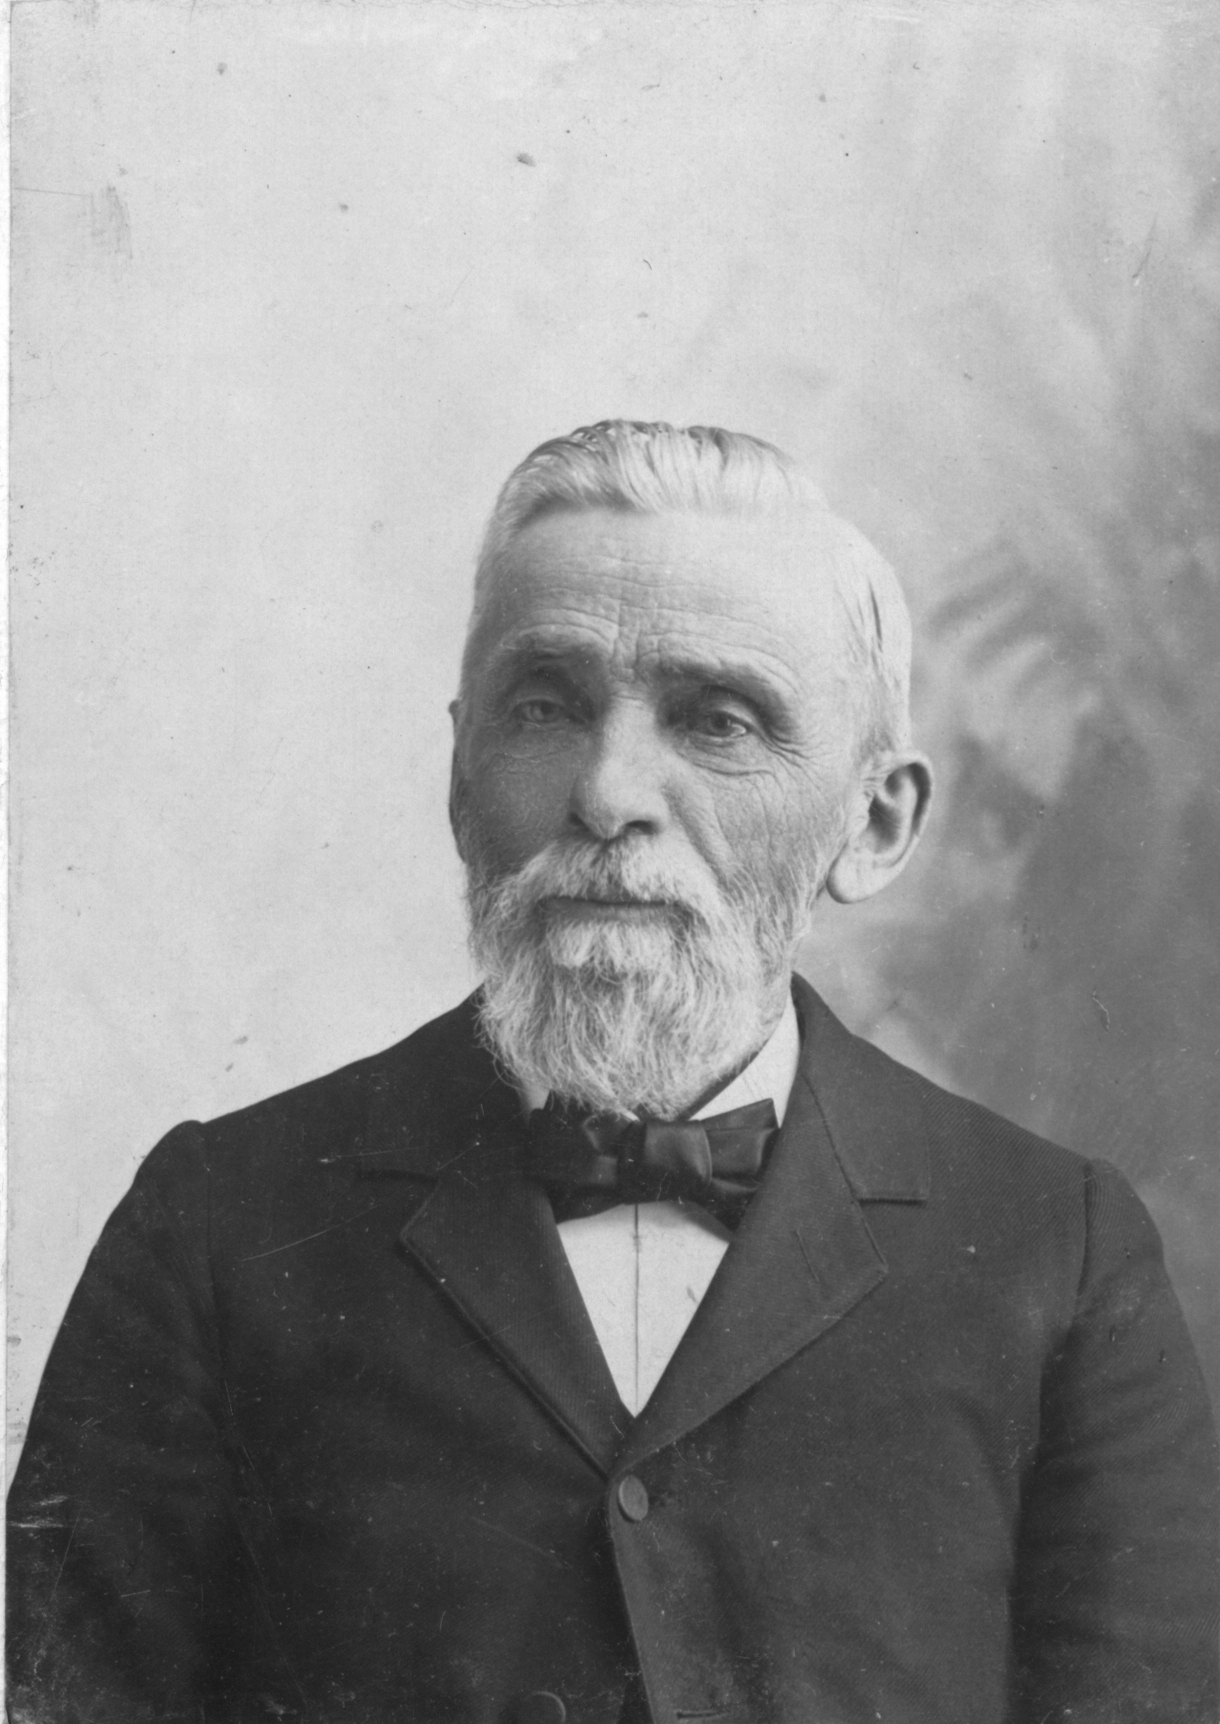
\includegraphics[width=1\linewidth]{images/john-n-loughborough.jpg}
    \caption*{John Norton Loughborough (1832-1924)}
    \label{fig:john-n-loughborough}
\end{figure}

\others{Što god bila istina po ovom pitanju, sigurno ne može biti pogrešno da istražimo što Riječ kaže o tome. \textbf{Mnogi se suzdržavaju od istraživanja nepopularnih istina jer se protiv njih diže optužba za herezu}. Ne smatramo se podložnima toj etiketi, \textbf{niti zadirujemo u tajne Svemogućeg dok nastavljamo s istraživanjem ove materije}. Biblija svakako sadrži svjedočanstva po ovom pitanju, i ponavljamo: ‘\textbf{Što je otkriveno, pripada nama}.’ Pitamo onda, što kaže Sveto pismo?}

\othersnogap{\textbf{Sâma svjedočanstva koja smo istraživali u vezi s činjenicom da je čovjek stvoren od praha zemaljskog na \underline{sliku Božju}, nedvosmisleno dokazuje da \underline{Bog ima oblik}, iako je to suprotno onome što smo učili kao djeca iz katekizma}:}

\othersnogap{Pitanje. Što je Bog?’}

\othersnogap{‘Odgovor. Beskonačni i vječni duh; onaj koji je uvijek bio i uvijek će biti.’}

\othersnogap{‘P. Gdje je Bog?’}

\othersnogap{‘O. Svugdje.’}

\othersnogap{\textbf{Ali pitamo, \underline{nije li Bog na jednom mjestu više nego na drugom}?} Oh ne, kažete vi: \textbf{Biblija kaže da je \underline{On duh}, i ako je tako, mora biti \underline{posvuda jednako prisutan}}. Po tome, znači, kada čovjek umre njegov duh ide Bogu, tada mora ići svugdje. \textbf{Ali Biblija svakako predstavlja Boga koji se nalazi na nebu. ‘Jer pogleda dolje sa svoje svete visine, GOSPOD s neba motri zemlju.’ Psalam 102:19}. \textbf{Onda svakako nebo ne može biti svugdje, jer se Bog prikazuje kako gleda odozgo. ‘\underline{Ilija uzađe} u vihoru \underline{na nebo}.’ 2. Kraljevima 2:11}. \textbf{Ali, kaže netko, zar Biblija ne prikazuje Boga kao \underline{sveprisutnog}?} Psalam 139:8, 9, 10. ‘Popnem li se na nebesa, \textbf{ti si ondje}; prostrijem li si postelju u Šeolu, \textbf{gle, ti si ondje}; uzmem li krila zorina pa se nastanim na kraju mora, \textbf{i ondje će me voditi ruka tvoja} i držat će me desnica tvoja.’}

\othersnogap{Mi odgovaramo, \textbf{odgovor je predstavljen u 7. retku, kako slijedi}: ‘\textbf{\underline{Kamo da odem od tvoga Duha}?} \textbf{i kamo da pobjegnem od \underline{tvoje prisutnosti}?}’ \textbf{Duh je \underline{Božji predstavnik}}. \textbf{Njegova sila se očituje gdje god On želi, kroz djelovanje Njegovog Duha}. Krist, kada je dao nalog učenicima, kaže: ‘Idite po svem svijetu i propovijedajte evanđelje svakom stvorenju, i evo! \textbf{ja sam s vama u sve dane do svršetka svijeta}.’ Sada, nitko ne bi tvrdio da je Krist bio osobno na zemlji otkako su učenici počeli ispunjavati ovaj nalog. \textbf{Ali njegov Duh je bio na zemlji; Tješitelj kojeg je obećao poslati.} \textbf{Tako se na isti način Bog očituje \underline{svojim Duhom} koji je također sila kroz koju On djeluje}. ‘A ako \textbf{Duh onoga} koji je uskrisio Isusa od mrtvih prebiva u vama, \textbf{onaj koji je uskrisio Krista} od mrtvih oživjet će i vaša smrtna tijela \textbf{\underline{po svome Duhu} koji prebiva u vama}.’ Rimljanima 8:11. \textbf{\underline{Ovdje je napravljena jasna razlika između Duha i Boga koji uskrisuje mrtve tim Duhom}}. \textbf{Ako je živi Bog Duh u najstrožem smislu te riječi, a istovremeno posjeduje Duha, onda odmah imamo neobičnu ideju o Duhu Duha, nešto što će trebati barem spiritualist da objasni}.}[The Adventist Review and Sabbath Herald, 18. rujna 1855][https://documents.adventistarchives.org/Periodicals/RH/RH18550918-V07-06.pdf]

Dopustite nam kratak komentar. Nadamo se da prepoznajete specifičnu temu o kojoj se ovdje raspravlja. Tema je prva točka \emcap{Fundamentalnih Principa} i tvrdnja da Bog ima oblik, jer je čovjek stvoren na Božju sliku. Takvo razumijevanje Božje ličnosti isključuje ideju da je Bog svugdje prisutan. Brat Loughborough je dao biblijske razloge za Božju sveprisutnost, zajedno sa sentimentom da je “\textit{Bog na jednom mjestu više nego na drugom}”. Bog je svugdje prisutan preko svog predstavnika, Svetog Duha, baš kao što je napisano u prvoj točki \emcap{Fundamentalnih Principa}. Dalje u ovoj raspravi, čitat ćemo da je Bog duhovno biće i posjeduje opipljivo, materijalno tijelo, za razliku od ideje da je On čisto duh.

\others{Postoji barem jedna nepremostiva teškoća na putu \textbf{onih koji vjeruju da je \underline{Bog nematerijalan}, i da nebo nije doslovno, \underline{locirano mjesto}: oni su prisiljeni priznati da je \underline{Isus tamo tjelesno, kao doslovna osoba}}; isti Isus koji je bio razapet, umro i pokopan, bio je uskrsnut iz mrtvih, \textbf{uzašao na nebo}, i sada je \textbf{s desne strane Boga}. \textbf{Isus je posjedovao tijelo i kosti nakon svojeg uskrsnuća}. Luka 24:39. ‘\textbf{Pogledajte moje ruke i moje noge, da sam to ja sam; opipajte me i vidite, }\textbf{\underline{jer duh nema tijela ni kostiju kao što vidite da ja imam}}.’ \textbf{Ako je Isus tamo na nebu s doslovnim tijelom od mesa i kostiju, možda je ipak nebo nakon svega doslovno mjesto, prebivalište za doslovnog Boga, doslovnog Spasitelja, doslovne anđele i uskrsnule besmrtne svete?} \textbf{\underline{Oh ne, kaže netko, ‘Bog je Duh.’}} Tako je Krist rekao ženi Samarijanki kod zdenca. \textbf{Ne slijedi nužno da zato što je Bog Duh, \underline{da nema tijelo}}. U Ivanu 3:6, Krist kaže Nikodemu, ‘\textbf{Što je rođeno od Duha, duh je}.’ \textbf{Ako je ono što je rođeno od Duha duh, onda po istom principu, ono što ima duhovnu narav je duh. Bog je \underline{duhovno biće}, njegova narav je duh, on nije smrtne naravi; \underline{ali to ne isključuje ideju da ima tijelo}}. David kaže, [Psalam 104:4,] ‘koji čini \textbf{svoje anđele duhovima};’ ipak \textbf{\underline{anđeli imaju tijela}}. Anđeli su se ukazali i Abrahamu i Lotu, i jeli su s njima. \textbf{Vidimo da ideja da su anđeli duhovi ne dokazuje da nisu doslovna bića}.}

\othersnogap{Zaključuje se, budući da Biblija kaže da je Bog Duh, da On nije osoba. Zaključak ne bi trebao biti temelj za argument. Velike biblijske istine su jasno navedene, i ne bi nam bilo dobro temeljiti doktrinu na zaključcima koji su \textbf{u suprotnosti s izričitim izjavama u Božjoj riječi}. Ako Pismo izričito \textbf{navodi da je Bog osoba, nije prikladno izvoditi zaključak iz teksta koji kaže ‘Bog je Duh,’ \underline{da On nema tijelo}}.}

\othersnogap{Sada ćemo predstaviti nekoliko tekstova \textbf{koji dokazuju da je Bog osoba}. Izlazak 33:18, 23. ‘I on (Mojsije) reče: Molim te, pokaži mi slavu svoju!’ Stih 20. ‘I reče: \textbf{Ne možeš vidjeti \underline{lice moje}, jer ne može čovjek vidjeti me i živjeti}.’ Stihovi 21-23. ‘I GOSPODIN reče: Evo, ima mjesto kod mene i ti ćeš stajati na stijeni. I dogodit će se, dok slava moja bude prolazila, da ću te staviti u pukotinu stijene i \textbf{zaklonit ću te \underline{rukom svojom} dok ne prođem}; i uklonit ću \textbf{ruku svoju}, i vidjet ćeš \textbf{\underline{leđa moja}}; ali \textbf{\underline{lice moje} neće se vidjeti}.’ \textbf{Ako je Bog \underline{nematerijalni Duh}, tada ga Mojsije nije mogao vidjeti; jer nam je rečeno da duh ne može biti viđen prirodnim očima}. \textbf{Tada ne bi bilo primjereno da Bog kaže da će staviti svoju ruku preko Mojsijeva lica dok prolazi (naizgled da ga spriječi da vidi Njegovo lice), jer ga ni nije mogao vidjeti}. \textbf{Niti možemo pojmiti kako bi nematerijalna ruka mogla spriječiti zrake svjetlosti da dođu do Mojsijevih očiju}. \textbf{Ali ako je tvrdnja istinita \underline{da je Bog nematerijalan}, i ne može biti viđen prirodnim okom, gornji tekst je potpuno suvišan}. \textbf{Kakvog smisla ima reći da je Bog stavio svoju ruku preko Mojsijeva lica, da ga spriječi od viđenja onoga što se ne može vidjeti}.}

\othersnogap{Kaže netko, vidim da ne možemo uskladiti stvar na drugi način, nego da je Mojsije vidio doslovno tijelo; ali to nije bilo Božje vlastito tijelo, \textbf{to je bilo tijelo koje je uzeo da bi se mogao pokazati Mojsiju}. \textbf{Mojsije nije mogao stvoriti ispravne predodžbe o Bogu osim ako On nije preuzeo neki oblik.} \textbf{Tako je Bog uzeo tijelo}. Ovo baca još goru sjenu na stvar nego prvi stav; \textbf{jer optužuje Boga za prijevaru; govoreći Mojsiju da će Ga vidjeti, dok prema ovom svjedočanstvu Mojsije zapravo nije vidio Boga, nego drugo tijelo}. Osoba mora sumnjati gotovo bez mogućnosti oporavka, koja bi pokušala tako mistificirati i poništiti snagu ovog svjedočanstva.}[Ibid.][https://documents.adventistarchives.org/Periodicals/RH/RH18550918-V07-06.pdf]

Prepoznajete li da se brat Loughborough bavi sentimentom koji će dr. Kellogg predstaviti u Živom Hramu 48 godina kasnije? Dr. Kellogg je rekao da je istina da se Bog predstavio u \others{\textbf{\underline{određenom obliku ili mjestu}}}[Dr. John H. Kellogg, The Living Temple, str. 31.][https://archive.org/details/J.H.Kellogg.TheLivingTemple1903/page/n31/] jer \others{mora postojati nešto \textbf{opipljivije}, više \textbf{\underline{ograničeno}}, na što se um može usredotočiti u bogoslužju}[bid, str. 30][https://archive.org/details/J.H.Kellogg.TheLivingTemple1903/page/n30/], ali da je On, u stvarnosti, \others{\textbf{daleko izvan našeg shvaćanja \underline{kao što su granice prostora i vremena}}}[Ibid, str. 33][https://archive.org/details/J.H.Kellogg.TheLivingTemple1903/page/n33/]. Brat Loughborough razumno se usprotivio ideji da se Bog samo manifestira čovjeku kao određeno Biće, ali u stvarnosti nije ono što se predstavlja da jest. Takva tvrdnja \others{optužuje Boga za prijevaru}. Brat Loughborough nastavlja s potvrdnim, biblijskim svjedočanstvom da je Bog materijalno biće.

\others{Izlazak 24:9. ‘Tada se popnu Mojsije i Aron, Nadab i Abihu, i sedamdeset starješina Izraelovih: \textbf{i vidješe Boga Izraelova}: i pod \textbf{njegovim nogama} bijaše kao pod od safira, i kao samo nebo po čistoći.’ Bilo im je dopušteno \textbf{vidjeti njegove noge}, ali nijedan \textbf{čovjek ne može vidjeti njegovo lice i živjeti}. \textbf{Nijedno \underline{smrtno oko} ne može podnijeti zasljepljujući sjaj te slave Božjeg lica}. Daleko nadmašuje sunčevu svjetlost. Jer prorok kaže: ‘Svjetlost mjesečeva bit će kao svjetlost sunčeva, a svjetlost će sunčeva biti \textbf{sedam puta jača}, kao svjetlost od sedam dana, u dan kad Gospodin zavije ranu svojega naroda i izliječi udarac njihove rane.’ Izaija 30:26. Unatoč toj sedmerostrukoj svjetlosti koja će tada sjati, prorok govoreći o tom prizoru kaže: ‘Tada će se mjesec zastidjeti i sunce posramiti, kad Gospodin nad vojskama zacaruje na gori Sionu i u Jeruzalemu, pred starješinama svojim u slavi.’ Izaija 24:23. Ivanovo svjedočanstvo je [Otkrivenje 21:23] ‘I grad ne treba ni sunca ni mjeseca da mu svijetle, jer \textbf{ga obasja slava Božja}, i njegovo je svjetlo Janje.’}

\othersnogap{\textbf{Nevjernici tvrde da postoji proturječnost u Mojsijevom svjedočanstvu, jer je rekao da je razgovarao s Bogom licem u lice}. \textbf{Odgovaramo, između njih je bio oblak}, ali Bog je rekao Mojsiju: ‘\textbf{Nijedan čovjek ne može me vidjeti i ostati živ}.’ Svjedočanstvo Novog zavjeta je u skladu s onim Starog zavjeta o ovom predmetu. ‘Težite za mirom sa svima i za posvećenjem, bez kojega \textbf{nitko neće vidjeti Gospodina}.’ Hebrejima 12:14. \textbf{Tko bi \underline{smrtnim očima} mogao gledati svjetlost koja sedam puta nadmašuje sjaj sunca?} Zasigurno nitko osim svetih ne može ga vidjeti, \textbf{samo besmrtne oči} mogu podnijeti tu blistavu slavu. Iako Riječ kaže da sada ne možemo vidjeti Boga i živjeti, obećanje je da će ga \textbf{čisti srcem vidjeti}. Matej 5:3. ‘Blago čistima srcem, \textbf{jer će Boga gledati}.’ Otkrivenje 22:4. ‘I \textbf{gledat će njegovo lice}, a njegovo će ime biti na njihovim čelima.’}

\othersnogap{Pavao [Kološanima 1:15] govoreći o Kristu, kaže: ‘On je slika \textbf{nevidljivoga Boga}, prvorođenac svakog stvorenja.’ Ovdje se za Krista kaže da je ‘\textbf{slika nevidljivoga Boga}.’ Već smo pokazali da \textbf{Krist ima tijelo sastavljeno od tvari, mesa i kostiju; i za njega se kaže da je} ‘\textbf{slika nevidljivoga Boga}.’ Pa dobro, kaže netko, priznajemo da je njegova božanska priroda na sliku Božju. Ako pod njegovom božanskom prirodom mislite na dio koji je postojao u slavi s Ocem prije postanka svijeta, odgovaramo, ono što je bilo u početku s Bogom (Riječ), \textbf{postalo je tijelo, nije ušlo u tijelo}, ili kako neki kažu, \textbf{zaodjenulo se ljudskom prirodom, nego postalo tijelo}. Ali kaže drugi, \textbf{za Boga se kaže da je nevidljiv}. \textbf{To što je sada nevidljiv, ne dokazuje da nikada neće biti viđen}. Riječ kaže: ‘Čisti srcem \textbf{vidjet će ga}’. Voljna vjera kaže, Amen.}

\othersnogap{Pavlovo svjedočanstvo u Filipljanima 2:5, 6, jasno pokazuje što se može razumjeti pod izjavom da je Krist slika Božja. ‘Neka u vama bude isto mišljenje kao i u Kristu Isusu: koji je \textbf{bio u obličju Božjem}, nije smatrao otimačinom \textbf{biti jednak Bogu}.’ \textbf{Kako se može reći da je Krist u obličju Božjem, ako Bog nema obličja?} Rimljanima 8:3. ‘Bog poslavši svoga vlastitog Sina u obličju grešnog tijela.’ \textbf{Krist je u obličju Božjem i u obličju ljudi. Ovo nam odmah otkriva obličje Božje}.}

\othersnogap{\textbf{\underline{Daniel govoreći o Bogu, naziva ga Pradavnim}}. Daniel 7:9. ‘I Pradavni sjede, \textbf{čija odjeća bijaše bijela kao snijeg}, i \textbf{kosa njegove glave} kao čista vuna.’ \textbf{Za ovu osobu se kaže da ima glavu i kosu; to se zasigurno ne bi moglo reći za njega} \textbf{\underline{kad bi bio nematerijalan i bez oblika}}. \textbf{Ali Pavlovo svjedočanstvo u \underline{Hebrejima 1:3}, trebalo bi riješiti svaku iskrenu sumnju u \underline{vezi ličnosti Boga}}. Govoreći o Kristu, on kaže: ‘Koji budući sjajnost slave njegove, \textbf{i savršena slika njegove (\underline{Očeve osobe})}.’ \textbf{Ovdje je jasno navedeno da \underline{Bog ima osobu}. Krist je savršena slika te osobe.} Tada možemo razumjeti Krista gdje kaže: ‘\textbf{Tko je vidio mene, vidio je Oca}.’ Ivan 14:19. \textbf{On nije mogao misliti da je on svoj vlastiti otac; jer kada se molio obraćao se svom Ocu kao drugoj osobi koja ga je poslala u svijet}. Nazivao se \textbf{Sinom Božjim}. \textbf{Stoga nije mogao biti Otac čiji je on bio sin}. Kada kaže: ‘Tko je vidio mene vidio je Oca,’ mora značiti da, kao što je \textbf{on bio savršena slika Očeve osobe, oni koji su vidjeli njega vidjeli su Očevu sličnost u njemu}.}[The Adventist Review and Sabbath Herald, 18. rujna 1855][https://documents.adventistarchives.org/Periodicals/RH/RH18550918-V07-06.pdf]

Važno je obratiti pažnju na biblijske dokaze koje brat Loughborough ističe u svjedočanstvu da Bog ima tijelo. Brat Loughborough pregledava nekoliko biblijskih odlomaka dokazujući da Bog ima materijalno tijelo, ali je nevidljivo našim smrtnim očima. Sestra White je napisala isto kada je rekla\egwinline{\textbf{Otac je sva punina Božanstva \underline{tjelesno}} i \textbf{nevidljiv je smrtnom pogledu}}. Nijedno smrtno oko ne može vidjeti Oca, ali to ne dokazuje da Bog nikada ne može biti viđen. Isus je rekao: \bible{\textbf{Tko je vidio mene, vidio je Oca}}[Ivan 14:19]. Isus je objasnio ove riječi dva poglavlja ranije: \bible{Isus povika i reče: Tko vjeruje u mene, ne vjeruje u mene, \textbf{nego u onoga koji me je poslao}. I \textbf{tko vidi mene vidi onoga koji me je poslao}}[Ivan 12:44-45]. Isus nije poslao samoga sebe, niti je Isus Otac, jedna te ista osoba; ali mi vidimo Oca u Kristu jer On je \textit{savršena slika Očeve osobe}. (Hebrejima 1:3). Kao što je Isus osoba, koja posjeduje tijelo, tako je i Otac. Brat Loughborough nastavlja dokazivati svoju poantu da je Bog osoba, koja posjeduje oblik i formu, jer je čovjek stvoren na Božju sliku.

\others{Ali sada ćemo se vratiti na temu stvaranja čovjeka. \textbf{Već smo vidjeli da to što je čovjek stvoren na sliku Božju, nije se moglo odnositi na moralnu sliku, jer bi to uključivalo apsurd da je beživotna glina od koje je čovjek oblikovan imala karakter poput Boga}. \textbf{Sada vidimo da Sveto pismo jasno uči da je \underline{Bog osoba s tijelom i oblikom}}. Tada se Postanak 1:26 može razumjeti da uči činjenicu \textbf{da je čovjek stvoren u obliku Božjem}. Drugi tekstovi se slažu s ovim svjedočanstvom. Vidi Postanak 9:6. ‘Tko prolije krv čovjekovu, njegovu će krv čovjek proliti: \textbf{jer na sliku Božju stvoren je čovjek}.’ \textbf{\underline{Ovo svjedočanstvo ne može se primijeniti na duh ili nematerijalni dio čovjeka: ono što je na sliku Božju ima krv}}. 1 Korinćanima 11:7. ‘Čovjek doista ne treba pokrivati glavu, \textbf{budući da je slika i slava Božja}.’ Jakov [Poglavlje 3:9] govoreći o jeziku kaže: ‘Njime blagoslivljamo Boga, Oca; i njime proklinjemo ljude \textbf{koji su stvoreni na sličnost (nalik, nalikovanje - Webster) Božju}.’ \textbf{Prethodno svjedočanstvo utvrđuje točku \underline{da se slika Božja ne odnosi na karakter nego na oblik}}.}

\othersnogap{Postanak 2:7. ‘\textbf{I Gospod Bog oblikova čovjeka od praha zemaljskoga i u nosnice mu udahnu dah života; i čovjek postade živa duša}.’}[The Adventist Review and Sabbath Herald, 18. rujna 1855.][https://documents.adventistarchives.org/Periodicals/RH/RH18550918-V07-06.pdf]

Bog je stvorio čovjeka na svoju sliku. Bog je osoba koja ima tijelo, oblik i formu, i On je stvorio čovjeka na svoju sliku. Iz ovog razmišljanja izvodimo očito značenje biblijskog svjedočanstva o \emcap{ličnosti Boga}. Ako stvorimo pogrešne koncepcije o Božjoj osobi, u opasnosti smo da pogrešno razumijemo druge istine koje su povezane s čovjekovom prirodom (smrtnost duše, stanje mrtvih, itd.). U svom članku, brat Loughborough nastavlja objašnjavati vezu između lažne doktrine o besmrtnosti duše i pogrešnih koncepcija o \emcap{ličnosti Boga}. Njegov članak u Review and Herald od 18. rujna, preuzet je iz njegove knjige “\textit{Ispitivanje Biblijskog Svjedočanstva}”\footnote{\href{https://egwwritings.org/?ref=en_MPC.2&para=961.2}{John Norton Loughborough, An Examination of the Scripture Testimony, 1855}}.

% Je li Bog osoba? - prema članku Johna N. Loughborougha

\begin{titledpoem}
    \stanza{
        Bog na prijestolju sjedi, kao osoba stvarna, \\
        Ne kao duh bez oblika, što je zabluda davna. \\
        Duhovno tijelo ima, iako našim očima skriveno, \\
        Previše sjajno za smrtnike, Pismom otkriveno.
    }

    \stanza{    
        Sveprisutan je Bog kroz Duha svog, \\
        Kao predstavnika moći, Lika tog. \\
        "Tko je vidio mene, vidio je Oca" - Krist zbori, \\
        Jer savršenu sliku Očeve osobe On tvori.
    }

    \stanza{
        Na Božju sliku stvoreni smo mi, \\
        U obliku, ne samo u naravi. \\
        Osoba prava s tijelom stvarnim jest, \\
        Ne magla bezoblična, kako neki žele svest.
    }

    \stanza{
        Bog jeste svepristuan, ali ne svugdje jednako, \\
        Na Nebu tijelom, a svugdje Duhom samo tako.
        Jednog dana čisti srcem će Ga vidjeti, \\
        Pred nogama Njegovim, će Ga obožavati.
    }
\end{titledpoem}
